%-------------------------------------------------------------------------------------------------%
% A related work section in which the relevant literature is presented and 
% linked to the project. 
% It should show that you clearly know the problem you plan to solve, 
% and that you master the related work. 

\chapter{Background}
\label{chap:background}

\begin{figure}
  \centering
  \graphicspath{ {../../assets/diagrams/} }
  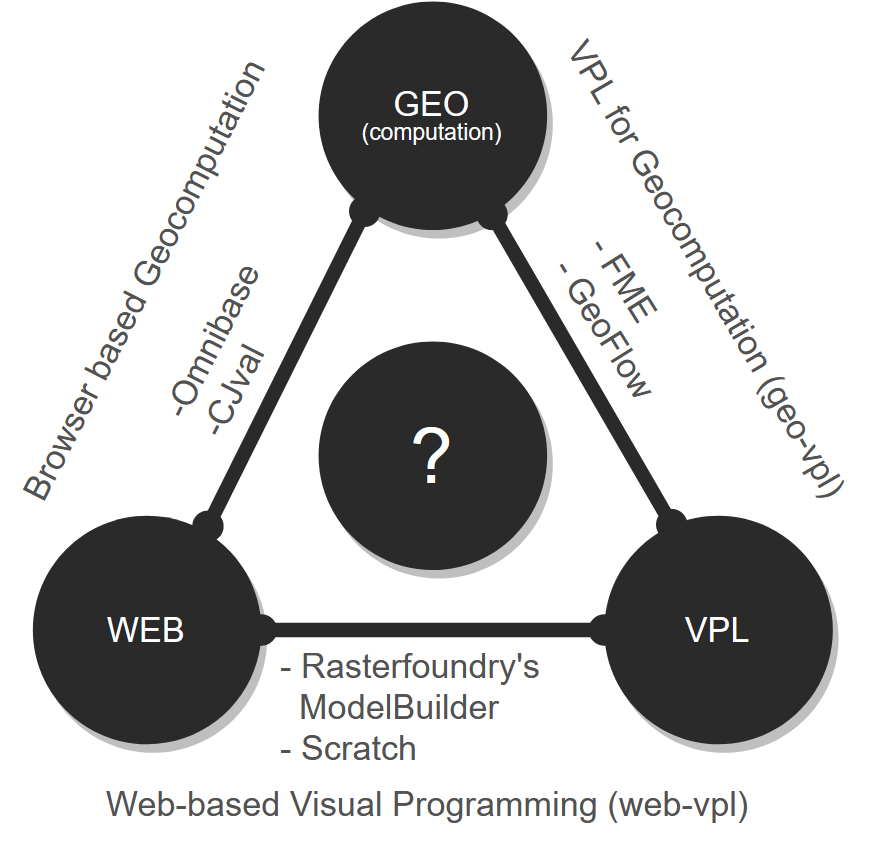
\includegraphics[width=270px]{geo-web-vpl.png}
  \caption{Triangle Model}
  \label{fig:triangle-model}
\end{figure}

This chapter offers an overview of the theoretical background that this study builds upon.
The study takes place at the intersection of three prior bodies of work,  represented by the corners of \reffig{fig:triangle-model}:
\begin{enumerate}[-]
  \item \refsec{sec:background-geo} covers the background on Geocomputation
  \item \refsec{sec:background-web} covers the background on Web applications
  \item \refsec{sec:background-vpl} covers the background on Visual Programming Languages
\end{enumerate}
Each one of these cornerstones will be discussed and analyzed by themselves, after which \refchap{chap:related} and \refchap{chap:methodology} will focus on the interplay and connections between these bodies of work. 

\section{Geocomputation}
\label{sec:background-geo}

\begin{note}
  TODO: finish this chapter
\end{note}

This section offers a brief background on the wide topic of geocomputation. 

% PURPOSE: Show that you understand geo-computation | Show why the rest of the study will focus on the computer graphics side of things

Geocomputation is a central component of the wider field of geo-informatics. 
The term geocomputation, or geodata processing, is used to represent all types of computations performed on geographical data. 
Anything from the calculation of an area of a polygon, to \ac{crs} transformations, feature overlay, or converting a raster dataset into a vectorized dataset, is regarded as geocomputation.

It must be emphasized that a geocomputational procedure is always fully defined by and dependent upon its input and output data types (similar to any type of computation). 
This is also why geocomputation is seldom a \emph{goal} in itself, but much rather the \emph{means} to discovering geo-information. 

\begin{note}
  TODO: show images of geo-computation
\end{note}

\subsection{Similarities and differences with neighboring fields}

\begin{figure}
  \centering
  \graphicspath{ {../../assets/diagrams/} }
  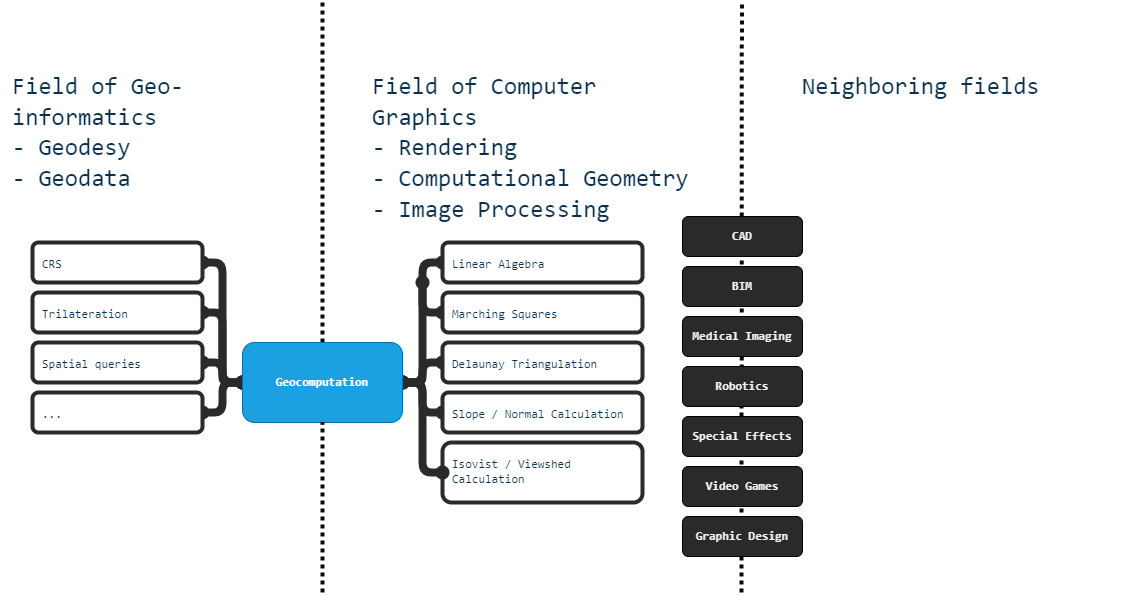
\includegraphics[width=380px]{geocomputation.png}
  \caption{Geocomputation in relation to other fields}
  \label{fig:geocomputation}
\end{figure}

Geocomputation can be seen as an applied field of the more general field of computer graphics. 
Other applications of computer graphics include computer aided design (CAD), Building Information Modelling (BIM), molecular biology, medical imaging, robotics, but also special effects, video games, and graphic design.
For this reason, these applied fields can be regarded as neighbors to geocomputation \& GIS. 

It is important to recognize that certain geocomputational procedures fully overlap with computer graphics and these neighboring fields, while others are very specific to the field of GIS and geo-informatics.
As an example, matrix transformations and reprojections are commonplace in the wider field of computer graphics, but transformations formalized and structured in the form of \ac*{crs} is very specific to the field of GIS (See \reffig{fig:geocomputation}).
As such, geocomputational procedures can roughly be categorized in two fields: 
\begin{itemize}[-]
  \item geocomputations \emph{specific} to \ac{gis},
  \item \emph{common} computational geometry procedures
\end{itemize}
This categorization can be identified by noting if an operation appears in a neighboring field, or just in the field of \ac{gis}.

This \emph{specific} category exists because of \ac{gis}s foundation in the field of Geodesy, and the nature of geographical data. 
Geodata differentiates itself from any form of data by its sizable nature, and geospatial nature. 
GIS dataset sizes easily scale into terabytes of data, and each datum specifically represent a real, measured, earthly phenomenon.
This makes storage and accuracy more relevant than other computer graphics applications. 

% NOTE TO SELF: GIVE CATEGORIES OF GEOCOMPUTATION IF IT IS ASKED FOR, OTHERWISE, LEAVE IT
% \subsection{Categories of Geocomputation}

% Geocomputation is a very broadly defined phenomenon, used to represent a great variety of computations. 
% To give an overview of this variety, a hierarchical subdivision of different types of geocomputation can be given, based on a subdivision of geodata types.

% The following distinctions are made between different geodata types:
% \begin{itemize}
%   \item Uniform
%   \subitem Rasters (Imagery)
%   \subitem Hexagons
%   \item Irregular, Vector-based
%   \subitem TIN 
%   \subitem solids
%   \subitem 3D Tiles
%   \item Semantic geodata:
%   \subitem Tabular geodata (QGIS)
%   \subitem Hierarchical, 'object oriented' geodata (GML / JSON) 
%   \item Point-cloud
% \end{itemize}

% Corresponding geocomputations are typically grouped together with one of these types of data. 
% However, this taxonomy is not perfect, since many computations exist \emph{between} between two different types of geodata.

% \subsubsection{Raster Geocomputation}

% - image processing
% - transformation kernels 

% \subsubsection{Vector Geocomputation}


% \subsubsection{Semantic Geocomputation}
% \begin{enumerate}[-]
%   \item often raster or vector at the core, with semantics layered on top 
% \end{enumerate}

% - 
% - 

% \subsubsection{Pointcloud Geocomputation}

\subsection{Geocomputation libraries}

\begin{figure}
  \centering
  \graphicspath{ {../../assets/images/background} }
  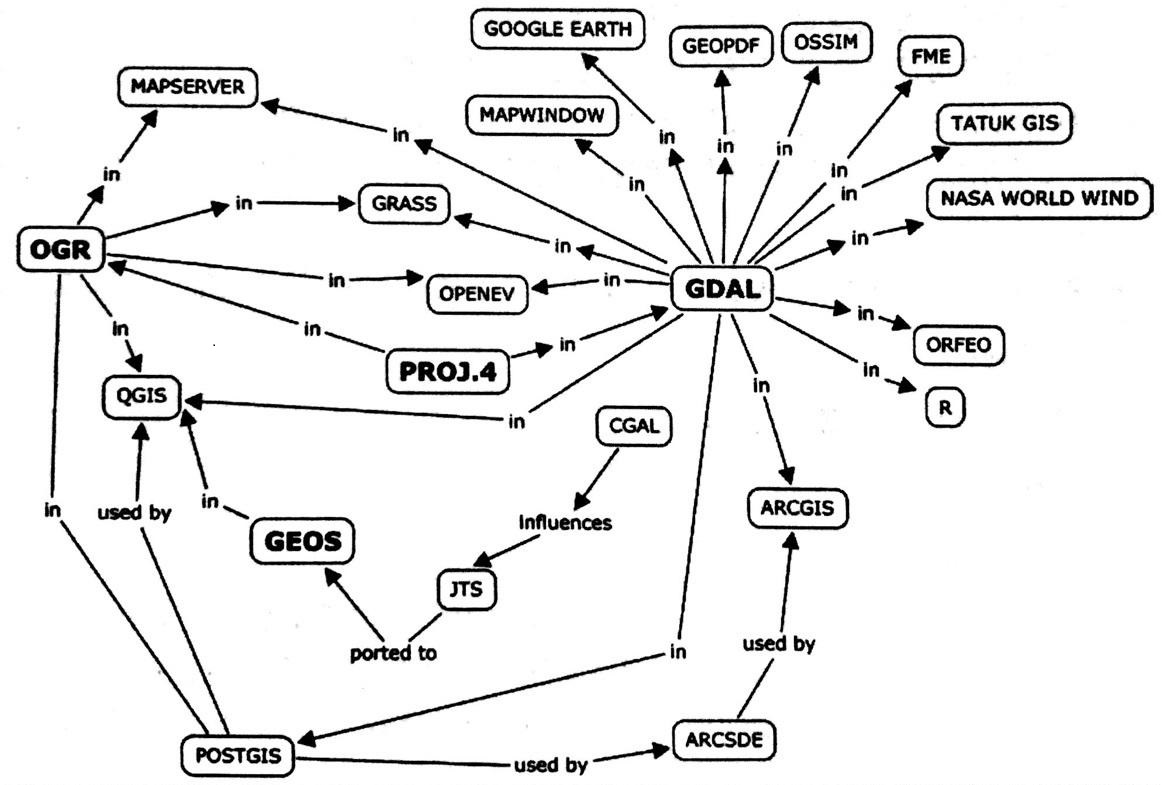
\includegraphics[width=380px]{all-geo-libraries-explained.jpg}
  \caption{Dependency graph of common geocomputation libraries. (This needs validation) }
  \label{fig:geolib-dependencies}
\end{figure}

Numerous geocomputational software libraries exist, written in a plethora of programming languages. 
Still, a certain 'Canon' can be defined based on popularity in terms of numbers of downloads, numbers of contributors, and number of dependent projects.  

Out of all open-source geocomputational libraries, the ones developed and maintained by the \ac{osgeo} (Source) can be regarded as the most significant to the field of \ac{gis}. 
These libraries include:
\begin{itemize}[]
  \item The \ac{gdal} (Source) 
  \item The Cartographic Projections and Coordinate Transformations Library titled PROJ (Source)
  \item The Geometry Engine Open Source (GEOS) (Source)
\end{itemize}
The geocomputations found in these libraries operate primarily on 2D / 2.5D raster and Simple Feature datasets (Source).
How these projects related together is presented by \reffig{fig:geolib-dependencies}.
Together, these libraries represent the core computational needs specific to the field of \ac{gis}. 

For the more common computational geometry needs, the \ac{cgal} library is also widely used.

% Almost all popular GIS end-user applications have these libraries at their core, such as 

\subsection{Conclusion}

The Take-away: 

Combination of general computational geometry, and computations very specific to GIS.

Geocomputation is mostly facilitated by a very select number of C++ libraries. 

\newpage

\section{Frontend web applications}
\label{sec:background-web}

\begin{note}
  TODO: this chapter is too large, the client-server / front-back elements should be trimmed down, or maybe even entirely removed. I think Its too granular. 

  Also, add more pictures!
\end{note}

This section offers a background on frontend web applications.
Since this topic is too large in scope to fully cover, three elements are chosen which are highly relevant to this study.
Finally, these three topics are linked to each other in \refsec{sec:background-web-conclusion}.

\subsection{Distributed systems}
\label{sec:background-web-terminology}

In software development of distributed systems, the following phrases exist: 
\begin{enumerate}[-]
  \item Client and Server 
  \item Frontend and backend
  \item Native application and web application
  \item web application and website
\end{enumerate}
While these phrases do overlap to an extend, years of interchangeable usage have lead to their differences often being overlooked. 
This study wishes to shed light on the relationships between these phenomena, as the nuances between them are vital to this studies contribution.

\subsubsection*{The client-server model}

\begin{figure}
  \centering
  \graphicspath{ {../../assets/images/misc/} }
  
\includegraphics[width=380px]{todo.jpg}
  \caption{A typical client-server interaction) }
  \label{fig:client-server}
\end{figure}

First, the client-server model. 
The client-server model refers to a distributed application architecture which balances storage and processing responsibilities between two cooperating types of programs: 
Clients and servers.
In this model, a client sends a request to a server, and the server provides the response asked for (see \reffig{fig:client-server}).
While this model immediately invokes images of web clients and web servers, it is important to recognize that the client-server model is far older than either web applications, or the World Wide Web in general. 
It is an abstract computational model, of which the World Wide Web is just one example.
A corresponding client and server may even exist on the same machine. 
A program running on a machine can act as a client, a server, or both, based on the role this program sets out to fulfill in relationship to other programs. 

The client-server model is beneficial for sharing resources, both in terms of storage and processing. 
A distinction is made between centralized models, in which the bulk of these resources are centralized on one or more servers, and decentralized models, which distribute and offload some or all of the computational resources to the clients. 
A centralized model has the advantage of making clients simple and interchangeable, at the cost of making them highly reliant on the uptake of and connection to the server. This also generates more client-server traffic. 
A decentralized model makes clients independent and decreases traffic, at the cost of the complications caused by decentralized architectures. 
The choice between a centralized or decentralized client-server model is therefore highly reliant on the resources of client and server hardware, as well as the quality of the connection between the server and client.  

\subsubsection*{Frontend and backend}

The terms frontend and backend, though closely related to clients and servers, refer to different phenomenon. 
Both are separations of concerns, a design principle prevalent in computer science to specialize a program into separate responsibilities. 
However, client and server programs are defined by their separation into "requester" and "responder" roles, whereas the frontend and backend are defined by their separation into "presentation" and "data access" functions. 
Presentation functions are responsible for interacting with the end-user of the application, and is concerned with aspects such as user interface, user interaction, and rendering.
"data access" interacts with the physical hardware of the machine, and is concerned with aspects such as storage methods, database management, and scalability.  
It just so happens that the presentation functions often corresponds with a requester role,
and that data access functions often corresponds with the responder role.
However, this is never a given. 
A server can be responsible for providing both the frontend and backend functionality, in the case the presentation of an application is rendered on this server. 

\subsubsection*{Native application and web application}

The nuances between a web application and a native application must also be specified, alongside their relationship to clients and servers. 
In this context, we make a distinction between \emph{Programs}, which refer to individual processes on either the side of the client or the server, and an \emph{application}, which either represents a non-distributed, self contained program, or represents the whole of corresponding client and server programs together.
Client programs or server programs are also often abbreviated as clients and servers.  
If a client runs without the corresponding server it relies upon, we can say that the client functions, but the entire \emph{application} does not function. 
In practice, however, the term 'web app' often specifically refers to the client, confusingly enough.

In any case, a program is considered native if it directly runs on the operating system of a device.
A program is considered web-based or browser-based if a browser is required to run it. 
A web application always has a client, as it will always need to be initially served by a corresponding server.
However, the extent to which the functionality of a web app is self contained or continuously reliant on this server may vary.
A native program may also be a client, as there is nothing preventing a native program of making the exact same web request as a web application. 

Due to this ambiguity of 'client-side' being able to refer to both native and web clients, this study makes use of the terminology 'browser-based programs' or 'browser-based applications', to point to web clients in particular. 

Web applications have specific advantages and disadvantages compared to native applications. 
The big advantages are that web applications are cross-platform by nature, and offer ease of accessibility, since no installment or app-store interaction is required to run or update the app (src: vpl 2019, src: hybrid).
As soon as a web app is found, it can theoretically be used.
The containerized nature of the web also makes web applications in general more safe. 
For unknown native applications there is always a danger of installing malicious software, whereas an unknown web application without any privileges is practically harmless (Needs citation). 
The ability to share the a functional application with a link, or to embed it within the larger context of a webpage, is also not a trivial advantage.

The disadvantage is that normally, web applications can only be written in JavaScript, a very-high level interpreted programming language. 
Its high-level nature leads to imprecision in using computational resources. 
For example, it makes no distinction between integer and floating point arithmetic.  
Additionally, the safety and containerization demands of the web make web applications more removed from the operating system and hardware.
Any type of \ac{os} interaction such as opening a window, interacting with the file system, or drawing directly to the screen buffer, is off-limits.  
Both these layers of indirection makes web applications traditionally unfavorable for demanding, highly specialized programs. 

\subsubsection*{Web application and website}

Lastly, a soft distinction is also made between websites, and web applications. 
Roughly speaking, a web application is a website which requires javascript in order to be functional.
This makes websites more static, and web applications more dynamic, being able to change based on user input.  
Wikipedia (Source) can be considered a website, whereas overleaf (Source) is definitively a web application. 
Many border cases also exist, like Twitter (Source).
Following the above definition, twitter is a web application, despite the fact that its core functionalities could be implemented without any client-side javascript.

\begin{note}
  Sources: 

  (https://en.wikipedia.org/wiki/Web_application, bad source, but this is more 'conventional wisdom' than true 'knowledge', couldn't find a more credible source, 
  
  what would make a person credible on this content?)
  
  (https://en.wikipedia.org/wiki/Frontend_and_backend)
\end{note}


\subsection{Rich Clients}
\label{sec:background-web-rich}

In the early days of the World Wide Web, web applications were practically impossible, and the web consisted of websites exclusively. 
Then, with the introduction of the javascript scripting language in 199x (Source), and browser plugins like Adobe Flash (Source), the first couple of web application slowly started to be developed. 
Still, these early web applications exclusively used a centralized client-server model.
The clients were simple, and completely reliant on the server. 

In the decades that followed, the javascript runtime of web browsers saw continuous improvements, alongside additions like HTML5, facilitating more interactive usage of webpages.
As the web and web technologies matures, new ways of using these technologies are discovered.
Web applications became more interactive, and frontend functionalities were slowly moved from the server to the client. 

These developments continued.
Since 2012, a trend of \textbf{rich web-clients} can be widely recognized \cite{hamilton_client-side_2014, panidi_hybrid_2015, kulawiak_analysis_2019}.
At that point, the browser had become powerful enough to allow for more decentralized client-server models.
By reducing servers to just static file servers, and adding all routing and rendering responsibilities to the client, the interactivity of a web application could be maximized. 
This model was dubbed "single page application", and was and still is facilitated by javascript frameworks like Angular, React and Vue.
However, the real facilitator of these developments are the browsers vendors themselves, as these frameworks would not be possible without the performance increase of javascript. 

This growth has also lead to web applications being used 'natively'. 
Tools like Electron (Source) allow web applications to be installed and 'run' on native machines by rendering them inside of a stripped down browser. 
Many contemporary 'native' applications work like this, such as VS Code, Slack, and Discord.
Additionally, tools like React Native (Source) are able to compile a web application into a native application without a browser runtime.  

If the applications resulting from both types of tools are to be regarded as 'web apps' or 'native apps', is left as an exercise to the reader. 
In any case, it becomes clear that rich web clients and their build tooling are starting to blur the line between native and web software.

\subsection{WebAssembly}
\label{sec:background-wasm}

If the line between web application and native application was already starting to get blurry, WebAssembly makes this line almost invisible. 
From all browser-based features, WebAssembly turned out to be a deciding factor of this study. This makes it important to be aware of the state of WebAssembly and its performance considerations.

\ac{wasm} is officially dubbed the fourth type of programming language supported by all major web browsers, next to HTML, CSS, and JavaScript.
Strictly speaking however, WebAssembly not a language, but a binary instruction format for a stack-based virtual machine.
(SOURCE: https://webassembly.org/)
it can be used to, theoretically, run any application or library in a web browser, regardless of the language used to create it, be it C/C++, Python, C\#, Java, or Rust. 
This means that in order to create a web application, developers can now in principle develop a normal, native application instead, which can then be compiled to WebAssembly, and served on the web just like any other web application. 

\subsubsection*{Limitations}

The sentence above uses the phrase \emph{in principle}, since there are quite a few caveats to the format. 
While in theory any application can be compiled to WebAssembly, in practice, not all applications turn into functional webassembly applications, due to certain factors.
These limitations can be split up into two groups: 
Limitations due to the web platform, and limitations due to the current state of the language and its host.

First of all, WebAssembly is required to adhere to the same containerization restrictions as javascript and the web at large. 
There is no '\m{os}' or '\m{sys}' it can call out to, as it cannot ask for resources which could be a potential security risk, like the file system.
Secondly, WebAssembly is in its early phases as a language, and is intended as a simple, bare-bones, low-level compile target. 
For example, the current version does not support concurrency features like multithreading.

Many of these shortcomings can be mitigated by calling JavaScript and HTML5 features from WebAssembly. 
This is what the majority of current WebAssembly projects look like. 
However, this layer of javascript 'boilerplate' or 'glue code' is inefficient, as it leads to duplication and redirection.
Additionally, platforms wishing to support WebAssembly must now also support javascript. 

\subsubsection*{Performance}

The initial performance benchmarks look promising. The majority of performance comparisons show that WebAssembly only takes 10\% longer than the native binary it was compared to \cite{haas_bringing_2017}. A later study confirms this by reproducing these benchmarks \cite{jangda_not_2019}. It even notices that improvements have been made in the two years between the studies. However, Jangda et. al. criticize the methodology of these benchmarks, stating that only small scale, scientific operations where benchmarked, each containing only 100 lines of code. The paper then continues to show WebAssembly is much more inefficient and inconsistent when it comes to larger applications which use IO operations and contain less-optimized code. These applications turn out to be up to twice as slow compared to native, according to their own, custom benchmarks. 
Jangda et. al. reason that some of this performance difference will disappear the more mature and adopted WebAssembly becomes, but state that WebAssembly has some unavoidable performance penalties as well. 
One of these penalties is the extra translation step, shown in \reffig{fig:wasm-trajectory}, which is indeed unavoidable when utilizing an in-between compilation target. 

Some studies have taken place evaluating \ac{wasm}'s performance for geospatial operations specifically. 
Melch performed extensive benchmarks on polygon simplification algorithms written in both javascript and WebAssembly \cite{melch_performance_2019}. 
It concludes by showing WebAssembly was not always faster, but considerably more consistent. 
Melch had this to say: "To call the WebAssembly code the coordinates will first have to be stored in a linear memory object. 
With short run times this overhead can exceed the performance gain through WebAssembly. 
The pure algorithm run time was always shorter with WebAssembly.". 
These findings match \cite{jangda_not_2019}, showing that the duplication of data into the webassembly memory buffer is a considerable bottleneck.

A recent study concerned with watershed delineation \cite{sit_optimized_2019} also concluded client-side WebAssembly to be more performant than server-side C, which, as a side effect, enabled their application to be published on the web without an active server. 

Lastly, the sparse matrix research of Sandhu et al. will be mentioned. \cite{sandhu_sparse_2018}. It shows again that WebAssembly's performance gain is most notable when performing scientific computations. it states: "For JavaScript, we observed that the best performing browser demonstrated a slowdown of only 2.2x to 5.8x versus C. Somewhat surprisingly, for WebAssembly, we observed similar or better performance as compared to C, for the best performing browser.". It also shows how certain preconceptions must be disregarded during research. For example, it turned out that for WebAssembly and JavaScript, double-precision arithmetic was more performant than single-precision, probably due to byte spacing.

Even though this study falls in the category of scientific computation, these performance considerations will still have to be taken into account. The most important conclusion to to take away from prior research on WebAssembly is that \ac{wasm} must not be regarded as a 'drop-in replacement', as \cite{melch_performance_2019} puts it. Just like any language, WebAssembly has strengths and weaknesses. While \ac{wasm} is designed to be as unassumptious and unopinionated about its source language as possible, the implementations of host environments do favor certain programming patterns and data structures over others, and this will have to be taken into account when using the compile target.

\begin{figure}[!tbp]
  \centering
  \begin{minipage}[b]{0.80\textwidth}
    \graphicspath{ {../../assets/images/misc/} }
    
\includegraphics[width=300px]{todo.jpg}
    \caption{Comparison of compilation trajectories}
    % based on the finding of \cite{jangda_not_2019}
    \label{fig:wasm-trajectory}
  \end{minipage}
\end{figure}

% \subsubsection{Background}

% The original paper on WebAssembly was published on June 14, 2017 \cite{haas_bringing_2017}. The authors write that the reason behind the creation of WebAssembly is the observation that certain web applications started using JavaScript as a compile target, using a high-performance subset of JavaScript called 'asm.js' \cite{mozilla_asmjs_2013}. However, JavaScript remains a high-level, highly abstract programming language, which never intended to be used as a compile target. The discrepancy between intended use and actual use led to many complications for developers using JavaScript this way, but also for the developers of JavaScript itself \cite{haas_bringing_2017}. 
% In order to relieve javascript of the responsibility of being a 'low-level' compilation target, developers of the four major browser vendors Mozilla, Google, Apple and Microsoft created WebAssembly and its corresponding paper, in a joined effort.

% This paper starts by promising WebAssembly as a save, fast, portable and compact compilation target. It continues by showing how previous attempts at low-level code on the web fail in at least one of these criteria, and that WebAssembly is the first to deliver on all of them. The follow up chapters cover a proof of memory safety, a proof of soundness of the language design, and the design decisions which had to be made to live up to those four criteria. These details will become relevant to the proposed thesis when reasoning about why WebAssembly might be faster in one case versus another.

% \subsubsection*{Adoption \& Implementation}

% not in a vaccuum

% On 5 December 2019, the \ac{w3c} officially pronounced WebAssembly as the fourth programming language of the web \cite{w3c_world_2019}. Philippe Le Hégaret, the \ac{w3c} Project Lead, writes “The arrival of WebAssembly expands the range of applications that can be achieved by simply using Open Web Platform technologies. In a world where machine learning and Artificial Intelligence become more and more common, it is important to enable high performance applications on the Web, without compromising the safety of the users,”. Since then, most major browsers have added official WebAssembly support.

% As of writing this proposal, WebAssembly has of yet not seen widespread adoption in web developer communities. Opinions deviate, but in general, WebAssembly is considered a niche technology, often being named as 'experimental' and 'bleeding edge'. 

% This would explain why, to the best of the author's knowledge, not many projects and papers explicitly link WebAssembly and GIS. Papers on \ac{wasm} do state \textit{"3d data transformations and visualization"} as some of the examples of a high performance web applications \cite{haas_bringing_2017, jangda_not_2019}. What's more, certain GIS applications, like Google Earth, have started to use WebAssembly, as seen in \reffig{fig:google-earth} \cite{google_google_2020}. How it is used is unknown due to the engine being closed-source, but it is speculated that \ac{wasm} is used to access code written for the original C++-based desktop application.

% \begin{figure}[!tbp]
%   \centering
%   \begin{minipage}[b]{0.80\textwidth}
%     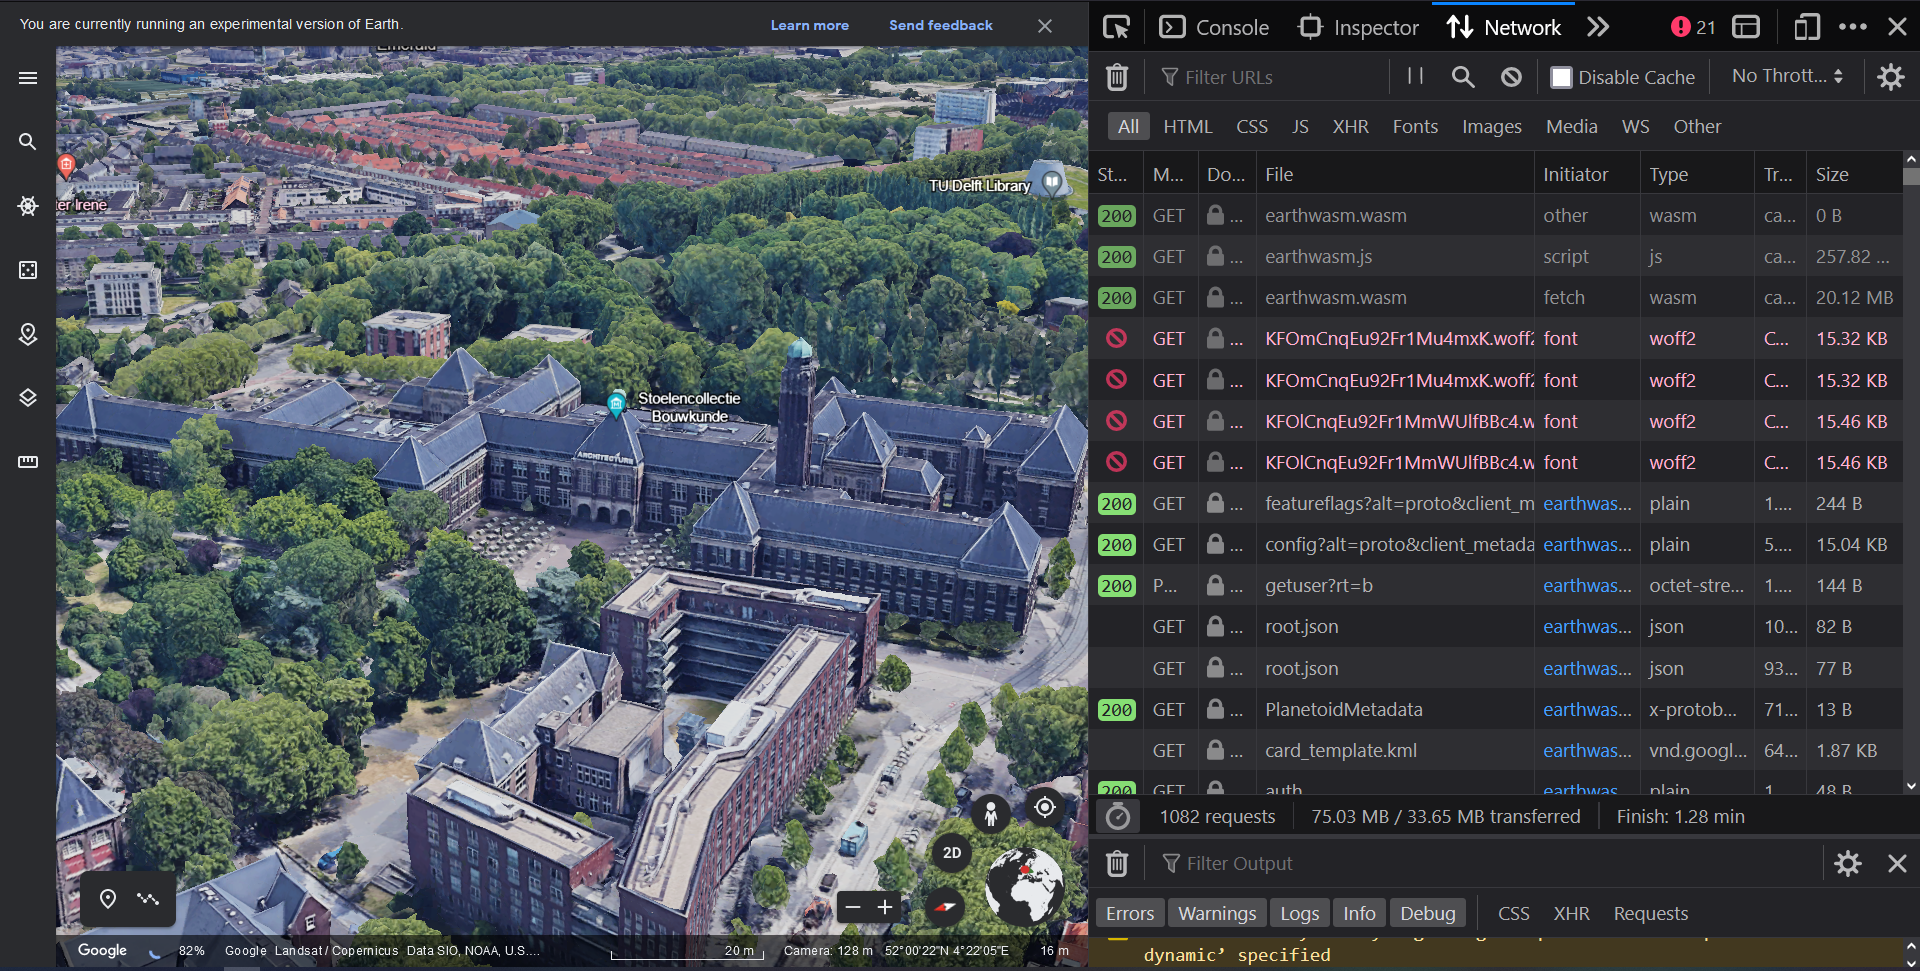
\includegraphics[width=\textwidth]{../images/google-earth-uses-webassembly.PNG}
%     \caption{Google Earth utilizing WebAssembly. Source: \cite{google_google_2020}}
%     \label{fig:google-earth}
%   \end{minipage}
% \end{figure}


% On the topic of WebAssembly, the most important conclusion to to take away from prior research is \ac{wasm} must not be regarded as a 'drop-in replacement', as \cite{melch_performance_2019} puts it. Just like any language, WebAssembly has strengths and weaknesses. While \ac{wasm} is designed to be as unassumptious and unopinionated about its source language as possible, the implementations of host environments do favor certain programming patterns and data structures over others, and this will have to be taken into account during the study.

%%%%%%%%%%%%%%%%%%%%%%%%%%%%%%%%%%%%%%%%%%%%%%%%%%%%%%%%%%%%%%%%%%%%%%%%%%%%%%%

% Based on the studies on WebAssembly, we can conclude that the compilation peculiarities of WebAssembly have to be taken into account, as it cannot be regarded as a 'drop in replacement'. There is also a significant difference between using WebAssembly theoretically, and using it realistically. The studies on Client-side geoprocessing tell us that these implementation details can have vast consequences on user experience, and studies on the Geoweb express that this user experience is vital to FAIR, cross-community geoprocessing.

% What this means for the methodology, is that a significant portion of this study's attention will have to go to experimenting with different ways of compiling to WebAssembly, while making sure it can still be used in a realistic scenario.
% If it turns out that the use-case app can only be used by experienced end-users who take special \ac{wasm} considerations in mind, a big reason of using the web, namely its accessibility, would be lost.  


%%%%%%%%%%%%%%%%%%%%%%%%%%%%%%%%%%%%%%%%%%%%%%%%%%%%%%%%%%%%%%%%%%%%%%%%%%%%%%%
% \subsubsection{(More on webassembly)}

% Not just open source: process sharing using fully containerized instances. Think .

% current vision / direction: containerized, sharable processes, together with web-based, front end visual programming environments ( RasterFoundry). Docker is usually named as a vision for these sharable processes.

% \m{->} We do have examples of cloud-native geodata formats, and some examples of cloud-based geo-computation (RasterFoundry , Google Earth Engine, more). However, these approaches have not yet tried to use truly sharable, containerized geoprocesses using Docker or WebAssembly. 

% \m{->} WebAssembly as a whole is underresearched. WebAssembly is not a fully virtualized container image, but just a binary set of instructions, meant to be executed on a virtual machine. Think of safe, cross-platform dll's. 
% WebAssembly is in this regard more simple than docker, but this gives it more opportunities. 
% WebAssembly runs in the browser for instance. 

% \m{->} This opportunity to run in the browser would enable these cloud-native frontend environments to "dry-run" these processes from within the browser, completely detached from the server, as a means to experiment with processes on a small scale before applying them to a cloud native environment. 

% \m{->} However, no implementations exist yet which combines containerized processes with these frontend computation environments. 

% # 2. BACKGROUND

% ## 2.1 The Web Browser & JavaScript
% -  main players (chrome, safari, firefox, edge(==chrome))
% - The browser js speed armsrace
% - How that lead to WebAssembly

% ## 2.2 The Geospatial Web. 
% [Still relevant]

% 2 biggest reasons against client-side geoprocessing: 
% - not performant enough
% - no equivalent to industry-standard libraries (CGAL / GDAL). 

% WebAssembly COULD solve both, so this study includes WebAssembly as 


% <br><br>

% .....

\subsection{Conclusion}
\label{sec:background-web-conclusion}

When reading \refsec{sec:background-web-terminology}, \refsec{sec:background-web-rich}, and \refsec{sec:background-wasm} together, a pattern emerges. 
WebAssembly blurs the line between the web-based and native development even further than the rich clients, and invites a further re-examination of our established models of distributed systems.
The compile target allows web-apps to make use of native libraries, and allows native software to be run on the web.
This second aspect offers a complete reverse workflow compared to the now popular Electron based applications described in \refsec{sec:background-web-rich}.
 
There was a significant initial delay between the improvements of the browser, and the widespread popularity of rich web clients. 
This study argues that as of right now, we are in the middle of a similar situation. 
A new technologies exist, it is implemented by all major browsers, and offers completely new ways of working with the web platform as a whole. 
The question remains what this will mean for the established models of clients and servers, the frontend and backend, and the web and native contexts. 

\newpage

\section{Visual Programmming}
\label{sec:background-vpl}

The third body of work this study draws from is works on the topic of visual programming. 
This section offers a brief overview on the topic itself, after which since \refsec{sec:related-geovpl} and \refsec{sec:related-webvpl} cover uses of visual programming in geocomputation and on the web, respectively. 

\subsection*{Visual programming languages}

A \ac{vpl}, or visual programming environment, is a type of programming language represented in a graphical, non-textual manner.
A VPL often refers to both the language and the \ac{ide} which presents this language in an editable way, by means of a \ac{gui}.
A visual programming language allows users to create programs by adding preconfigured components to a canvas, and connecting these components to form programs. 

Multiple types of \ac{vpl}s exist, but also multiple taxonomies of these types.
This study bases itself on the classifications presented in \cite{kuhail_characterizing_2021}, stating four different types of visual programming languages: 
\begin{enumerate}
  \item \textbf{Block-based languages}, in which all normal programming language features, like brackets, are represented by specific blocks which can be 'snapped' together (\label{fig:sidebyside:1}).
  \item \textbf{Diagram-based languages}, in which programming function are represented by nodes, and variables are represented by edges between these components (\label{fig:sidebyside:2}). This makes the entire program analogous to a Graph.
  \item \textbf{Form-based languages}, in which the functioning of a program can be configured by means of normal graphical forms (\label{fig:sidebyside:3}). 
  This approach enhances the stability and predictiveness compared to other types, at the cost of expressiveness.
  \item \textbf{Icon-based languages}, in which users are asked to define their programs by chaining highly abstract, iconified procedures (\label{fig:sidebyside:4}). 
\end{enumerate}

The meta analysis of \cite{kuhail_characterizing_2021} shows a great preference among researchers for block- and diagram-based languages. 
Only 4 out of 30 of the analyzed articles chose a form-based vpl, and only 2 chose an icon-based approach.  

This study wishes introduce a fifth type of VPL. 
A \textbf{Dataflow} VPL is a subtype of a diagram based VPL which only uses pure functions as computation nodes, only uses immutable variables, and which disallows cyclical patterns. This makes this VPL not only a graph, but a \ac{dag}.
More on this in \refsec{sec:background:dataflow}.

\begin{figure}
\centering
\begin{subfigure}[b]{0.45\linewidth}
  \graphicspath{{../../assets/images/background/vpl/}}
  \centering
  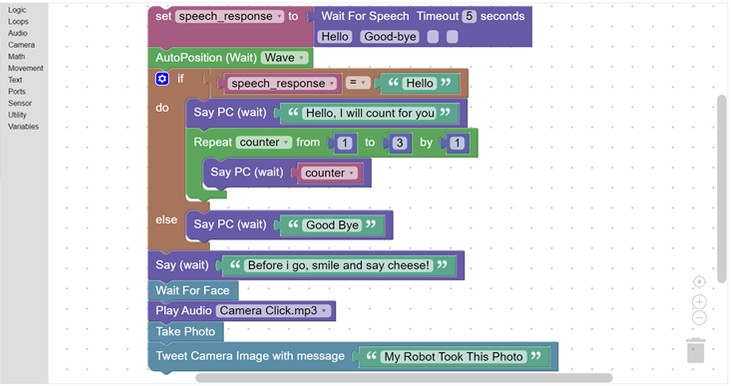
\includegraphics[width=\linewidth]{block-based.png}
  \caption{}\label{fig:vpl-types:1}
\end{subfigure}%
\qquad %-- that adds some space between th 2 figures
\begin{subfigure}[b]{0.45\linewidth}
  \graphicspath{{../../assets/images/background/vpl/}}
  \centering
  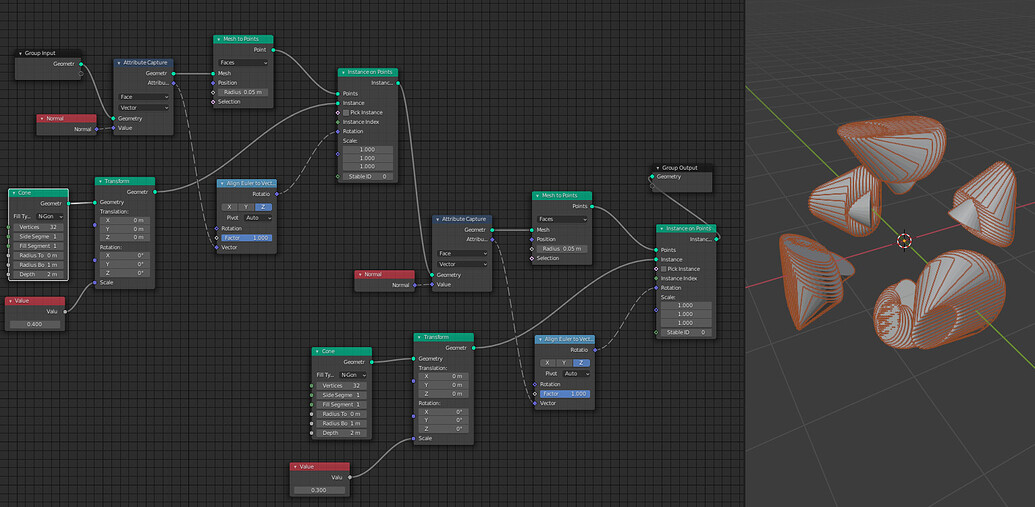
\includegraphics[width=\linewidth]{diagram-based.jpg}
  \caption{}\label{fig:vpl-types:2}
\end{subfigure}%
\\
\begin{subfigure}[c]{0.45\linewidth}
  \centering
  \graphicspath{{../../assets/images/background/vpl/}}
  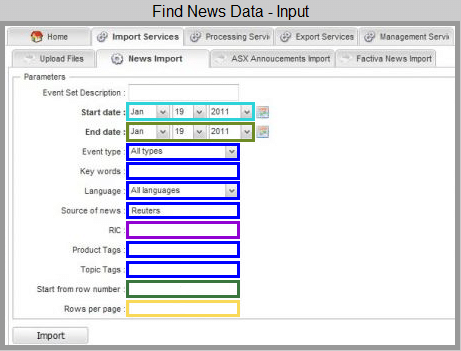
\includegraphics[width=\linewidth]{form-based.png}
  \caption{}\label{fig:vpl-types:3}
\end{subfigure}%
\qquad %-- that adds some space between th 2 figures
\begin{subfigure}[d]{0.45\linewidth}
  \centering
  \graphicspath{{../../assets/images/background/vpl/}}
  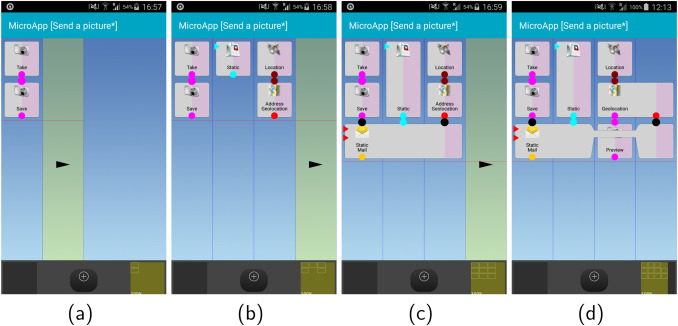
\includegraphics[width=\linewidth]{icon-based.jpg}
  \caption{}\label{fig:vpl-types:4}
\end{subfigure}%
\caption[Types of \ac{vpl}s]{Four different types of visual programming languages: Block-based, diagram-based, form-based, and icon-based, respectively}%
\label{fig:vpl-types}
\end{figure}

Visual programming languages are used in numerous domains. 
The vpls of the 30 studies examined by (SOURCE) were aimed at domains such as the Internet of Things, robotics, mobile application development, and augmented reality. 
Within the domain of systems control and engineering, The Ladder Diagram vpl (SOURCE) is the industry-standard for programming Programmable Logic Controllers (PLCs).
\ac{vpl}s are also widely used within computer graphics related applications, including the field of \ac{gis}, 
These will be covered in \refsec{sec:related-geovpl}.
Lastly, \ac{vpl}s also have great educational applications. 
Harvard's introduction to computer science course, CS50, famously starts out with Scratch, a block-based visual programming language normally targeted at children, to teach the basics of computational thinking (Source: CS50). 

% \begin{note}
%   Traditionally, visual programming has been successfully used to help novices
%   learn basics of programming by visualizing elements of a program. 
%  However, visual programming is increasingly being used by end 
%  users in various domains to create and tailor applications that are useful 
%  beyond the realm of education. 
%  For instance, VPLs are now being used in fields such as 
%  the 
%  From characterizing_2021
 

\subsection{Usability}

Studies on \ac{vpl}s indicate that generally speaking, VPLs make it easy for end users to visualize the logic of a program, and that vpls eliminate the burden of handling syntactical errors \cite{kuhail_characterizing_2021}.

The locally famous Cognitive Dimentions study \cite{green_usability_1996}, states that \emph{"The construction of programs is probably easier in VPLs than in textual languages, for several reasons: 
there are fewer syntactic planning goals to be met, such as paired delimiters, discontinuous constructs, separators, or initializations of variables; 
higher-level operators reduce the need for awkward combinations of primitives; 
and the order of activity is freer, so that programmers can proceed as seems best in putting the pieces of a program together."}. 
Indeed, a vpl UI can be used to eliminate whole classes of errors on a UI level by, for example, not allowing the connection of two incompatible data types. 

\begin{note}
  TODO: this is a weak argument. This also needs to be more nuanced
\end{note}

% //The meta analysis of \cite{kuhail_characterizing_2021} also 

These properties together make visual programming also highly suitable for activities of \textbf{experimentation} and \textbf{debugability}, and not only for end users. 

% ADVANTAGE: PLAYFULNESS

\subsection{End User Development \& Low Coding}
a \ac{vpl} done right can make automation available to a very large audience, and this is exactly the point. 
Visual Programming is part of a larger field, named End User Development (eud). 
The field is concerned with allowing end users who are not professional software developers to write software applications, using specialized tools and activities. 
This however, does not mean that experienced developers have nothing to gain from this research. 
Lowering the cognitive load of certain types of software development could save time and energy which can then be spend on more worthwhile and demanding tasks. 

\cite{kuhail_characterizing_2021} point out two serious advantages of EUD. 
First, end users know their own domain and needs better than anyone else, and are often aware of specificities in their respective contexts (\cite{kuhail_characterizing_2021}). 
And two, end users outnumber developers with formal training at least by a factor of 30-to-1 according to Kuhail et. al., and my suspicion is that this might be much higher.

% rewrite this more professionally...
I would like to add that offering the general public a chance to automate repetitious workflows might not only increase productivity, but can also greatly improve the quality of life in general, by focussing on the profound instead of the mundane. 

In the private sector, \ac{eud} is represented by the "low code" industry. 
Technology firms such as Google and Amazon are investing at scale in low-coding platforms (\cite{kuhail_characterizing_2021}),
The market value was estimated at 12.500 Million USD (Source: ), and with a growth rate between 20 and 40 percent, the value may reach as high as 19 Billion by 2030 (SOURCE: FORRESTER) 

\subsection{Dataflow programming}
\label{sec:background:dataflow}
An important aspect of the dataflow-VPL is the connection to the field of dataflow programming, which is not necessarily linked to VPLs. 

Dataflow programming is a programming paradigm which internally, represents a program as a \ac{dag} (SOURCE Dataflow 2012). 
A graphical, editable representation of a dataflow program would result into a Dataflow \ac{vpl}.

The big computational advantage of this model, is that it allows for implicit concurrently (SOURCE dataflow 2012). 
In other words, every node of a program written using dataflow programming can be executed in isolation of any other nodes, as long as the direct dependencies (the inputs) are met. 
No global state or hidden side effects means no data-race issues, which allows parallel execution of the program by default.
When using other paradigms, programmers need to manually spawn and manage threads to achieve the same effect. 

This leads into an interesting side-effect of using dataflow programming / a diagram-based \ac{vpl}: 
By only permitting pure, stateless functions with no side-effect, and only immutable variables, end users automatically adopt a functional programming style (albeit without lambda functions).
Functional programming has many benefits of its own besides concurrency, such as clear unit testing, hot code deployment, debugging advantages, and lending itself well for compile time optimizations (SOURCE: functional programming).


% functional programming

% Spreadsheets are probably the most common example of DFP
% and widely adopted by every type of computer users.
% On a spreadsheet, each cell represents a node that can either be an expression
% or a single value. Dependencies can exist to other cells. Following the dataflow
% model, whenever a cell gets updated, it sends its new value to those who depend
% on it, that update themselves before also propagating their new values. This
% specific type of application is commonly denominated as Cell-Oriented DPF or
% Reactive programming.

The important take-away is this: 
A \ac{vpl} is not just a matter of a user-friendly UI or a stylistic choice.
This might be true for block-based vpls, but not for diagram-based vpls. 
By closely resembling dataflow itself, and because of its functional programming nature, diagram-based vpls can actually lead to faster and more reliable software.

\subsection{Disadvantages and open problems}
\label{sec:background:vpl:disadvantages}

there is of course, no such thing as a free lunch. 
\ac{vpl}s and dataflow programming en large have got certain disadvantages and open problems.

% (Dataflow programming is an area still open to further research, with some open
% issues to answer. In fact, most of the open questions today have long been
% identified and despite the improvements, patterns for answering them are yet to
% be achieved.)

% block-based visual programming: just purely UI, diagram-based vpl add additional, functional programming qualities. 


\subsubsection*{Iteration and conditionals}

\begin{figure}
  \centering
  \begin{subfigure}[b]{0.45\linewidth}
    \graphicspath{{../../assets/images/background/vpl/}}
    \centering
    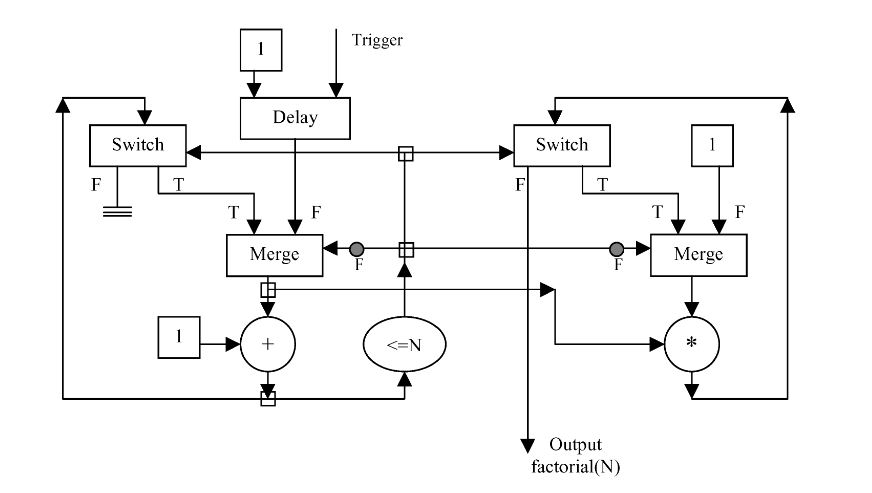
\includegraphics[width=\linewidth]{iteration-vpl.png}
    \caption{}\label{fig:vpl-iteration:1}
  \end{subfigure}%
  \qquad %-- that adds some space between th 2 figures
  \begin{subfigure}[b]{0.45\linewidth}
    \graphicspath{{../../assets/images/background/vpl/}}
    \centering
    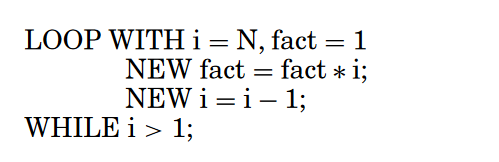
\includegraphics[width=\linewidth]{iteration-text.png}
    \caption{}\label{fig:vpl-iteration:2}
  \end{subfigure}%
  \caption[Comparrison of iteration]{A factorial function, written in a vpl, and textual form}%
  \label{fig:vpl-iteration}
  \end{figure}

A problem described in almost all reviewed vpl literature (Source: advanced in dataflow, SOURCE: Dataflow programming,  SOURCE: COGNITIVE), is that the \ac{dag} model of diagram-based vpls are ill-suited for representing even the most basic flow control statements: \m{if, else, for, while}.
Even if the acyclic quality of the dataflow graph is omitted, the resulting models are significantly more complicated compared to their textual counterparts, as shown by \reffig{fig:vpl-iteration}.

\subsubsection*{Encapsulation \& reusability}
Similar and yet different is the topic of encapsulation, or, how (SOURCE: COGNITIVE) names this problem: 'visibility'.
It is widely known that as a program scales in size, the complexity of handling the application scales exponentially.
In textual languages, reducing this complexity is often achieved by means of encapsulating sub-routines and re-usable parts of the program into separate functions.
Inner functionality is then hidden, and operations can be performed on a higher level of abstraction. 
This hierarchy of abstraction is just as achievable for \ac{vpl}s as described by (SOURCE: Dataflow programming).
However only a select number of \ac{vpl}s offer a form of encapsulation, and even less allow the creation of reusable functions, or creating reusable libraries from vpl scripts.
It appears that \ac{vpl} researches and developers are either not aware of the importance of encapsulation, or have encountered problems in representing this feature in a graphical manner.

% \subsubsection{High viscocsity}
% Viscosity was surprisingly high in the languages we looked at. The role of the diagram editor is crucial, yet few research papers in the usual programming literature discuss the design of effective diagram editors. In our straw viscosity test we found a range from about 1 minute to about 9 minutes for making semantically equivalent changes to programs in different languages. Visibility can be very poor. Systematic, easy-to-understand search tools need to be developed and user-tested, and if at all possible de facto standards should be adopted.

\subsubsection*{Subjective Assessment}
Additionally, the claims that \ac{vpl}s lend themselves well for end-user development is problematic from a technical perspective. 
Usability is a nebulous phenomenon, and challenging to measure empirically.
As often with more subjective matter, researchers have yet to form a consensus over a general evaluation framework. 
There is, however, a reasonable consensus on the 'qualities' a VPL should aspire to. 
This is different from a full assessment framework, but nontheless useful for comparing \ac{vpl}s.
The dimensions given in the cognitive dimensions framework (SOURCE) have acquired a somewhat canonical nature within \ac{vpl} research.
The number of citations of this work is relatively high, and indeed, almost all \ac{vpl} studies the author was able to find referred back to this critical work.   
In so far as this study needs to address the usability of the prototype VPL, we will thus follow this consensus, and base any assessment on (SOURCE).

% - we will make no such attempt. usability serves as background motivation. 
% - this study assumes vpl's are 'in general' more usable to end-users 
% than text-based alternatives, based on the positive results of most of the 
% studies analysed by communicating_2021.

\subsubsection*{Lacking Life-cycle support}
Finally, (communicating 2021) names the 'life cycle' of applications created by \ac{vpl}s as one of the most overlooked aspects within VPL research.
Out of the 30 studies covered by the meta analysis, only one briefly touched the topic of life cycle. 
Life cycle in this context refers to all other activities besides "creating an application that does what it needs to do".
Examples of these activities are version control, extending an existing application, debugging, testing the codebase, and publishing the application to be used outside of an \ac{ide}. 
These operational aspects are critical to making any application succeed, and \ac{eud} research should not be limited to purely the aspect of creating functionalities.

This oversight on life-cycle aspects can be found in the \ac{vpl} \& low-coding industry as well. 
\begin{note}
TODO: Formalize these ramblings, or don't. 

- no existing VPL ( that I know of ) has proper git-based version control. 
  - Most vpls use proprietary storage and collaboration methods. 
- vpls which are able to compile to a textual format are rare
  - vpls able to compile to a programming language, or a headless format, are even more rare. 

- Let alone: on operational programming paradigms such as Test driven development (TDD), continuous integration (CI), continuous delivery (CD).  

- in general, the life-cycle support of most vpls found in the low-coding industry are closely tied to their business models. 
  - Users can only use the publication tools, version control tools, and package / library managers offered to them by the vendor.

\end{note}

And while we are on the topic of publication, only 16 out of 30 of the tools analysed by (communicating 2021) were available publicly with some documentation.
It seems the lack of publication tooling might also partially be due to a lack of publication in general. 

\subsection{Conclusion}

The background literature clearly indicates many advantageous properties of vpls, both in terms of (end) user experience and the dataflow programming properties. 
Additionally, the studies showed important considerations which have to be taken into account in the design of any vpl.  
Lastly, the studies agree on several open-ended issues of which a satisfying answer is yet to be found. 

%%%%%%%%%%%%%%%%%%%%%%%%%%%%%%%%%%%%%%%%%%%%%%%%%%%%%%%%%%%%%%%%%%%%%%%%%%%%%%%
%%%%%%%%%%%%%%%%%%%%%%%%%%%%%%%%%%%%%%%%%%%%%%%%%%%%%%%%%%%%%%%%%%%%%%%%%%%%%%%
%%%%%%%%%%%%%%%%%%%%%%%%%%%%%%%%%%%%%%%%%%%%%%%%%%%%%%%%%%%%%%%%%%%%%%%%%%%%%%%
